\section{Extending Electron Coherence}

To be able to resolve and address weakly coupled carbons it is necessary to extend the coherence of the NV-spin.
By using a technique known as a spin-echo variations between experiments can be eliminated, making variations during experiments the main source of decoherence.
By dynamical decoupling the effect of these variations on the coherence can be minimized and the dynamics of the spin-bath exposed.


\subsection{Spin-Echo}



A spin echo experiment (\cref{fig:spin_echo_gijs}) is very similar to a Ramsey experiment.
An additional $\pi$ pulse is added in the middle of the experiment exactly between the $\pi/2$ pulses of the Ramsey sequence.
In a spin echo the state is brought into the XY-plane where it evolves for a time $\tau/2$ before a $\pi$-pulse, along the y-direction in the rotating frame, is applied.
It evolves for another $\tau/2$ before a final $\pi/2$-pulse rotates it back to $\ket{0}$ and it is read out.

\begin{figure}[htbp]
    \centering
    \includegraphics{Img/SpinEcho_Gijs.pdf}
    \caption{Spin Echo experiment }
    \label{fig:spin_echo_gijs}
\end{figure}

The $\pi$-pulse can be seen as turning the reference frame of the NV-spin upside down.
If the environment does not change during the experiment the detuning of the evolution frequency with respect to the central frequency during the first part will be exactly opposite to the detuning during the second part.
This means that any phase difference picked up during the first half of the evolution is canceled out perfectly during the second half of the evolution.

Because the spin-bath does not remain static during experiments the cancellation is not perfect causing some phase to be picked up causing decoherence.
Similar to a Ramsey experiment this can be measured by applying a detuning to the rotating frame and measuring the decay of the oscillation.
$T_2$ is defined as the $1/e$ value of the decay of a spin echo experiment and measures decoherence due to variations in the spin-bath during an experiment.
$T_2$ was measured to be $1.10 \pm 0.01 ms$.
% Data from exp:  20140405/123712

\subsection{Dynamical Decoupling}


A natural way of extending the short timescale behavior of the spin-echo to longer timescales is by applying more $\pi$-pulses. This procedure known as dynamical-decoupling can dramatically improve coherence times by decoupling the central-spin from the environment\citep{Lange2010Universal}.

Although dynamical-decoupling improves the coherence of the central spin by decoupling from the environment, the central spin is also decoupled from other spins preventing direct two-qubit gates. It was demonstrated by \citet{Sar2012DecoherenceProtected} how to incorporate dynamical decoupling in a universal gate design by implementing Grover's algorithm.
Using this technique \citet{Taminiau2012Detection} used the extended coherence to detect and control weakly-coupled carbon spins, before implementing three-qubit quantum-error-correction (QEC) \citep{Taminiau2014Universal}.

As these experiments where performed with NV-centers at Room temperature they lack the option to do single-shot readout required to act on a measurement outcome\footnote{@Tim, I think this can be worded more concisely. Do you have any ideas?}. An essential feature for the parity measurements that form the basis of measurement-based QEC and surface codes.

\subsection{Dynamical decoupling spectroscopy}
As we cannot perform an ESR experiment while decoupling a different technique must be used to resolve and address additional spins.
In order to resolve additional spins we perform a dynamical decoupling spectroscopy, resulting in a fingerprint of the nuclear-spin environment\citep{Taminiau2012Detection}.

In a dynamical decoupling spectroscopy experiment the electron is prepared in the $|X\rangle = |0\rangle +|1\rangle$ state. It is subjected to a decoupling sequence consisting of N/2 blocks of the form {$\tau - \pi -2\tau-\pi-\tau$}, and concluded by measuring $\langle X\rangle $. The fingerprint is the result of many repetitions for a range of inter-pulse delays $2\tau$. $\pi$ is a $\pi$-pulse.

Part of a dynamical decoupling spectroscopy can be seen in \cref{fig:FP}. The spectroscopy was performed for N = 8, 16, 32 and 64 pulses. For N = 8, 16 and 32 pulses this was done between $\tau = 2 \mu \mathrm{s}$  and $72 \mu \mathrm{s}$ and for N = 64 this was done up to $\tau = 52 \mu \mathrm{s}$. A reference to the full spectroscopy can be found in \cref{chap:Fingerprint_data_appendix}.

\begin{figure}[htbp]

    \begin{subfigure}[t]{\textwidth}\centering
        \caption{}
        \begin{tikzpicture}
            \node[anchor=south west,inner sep=0] at (0,0) {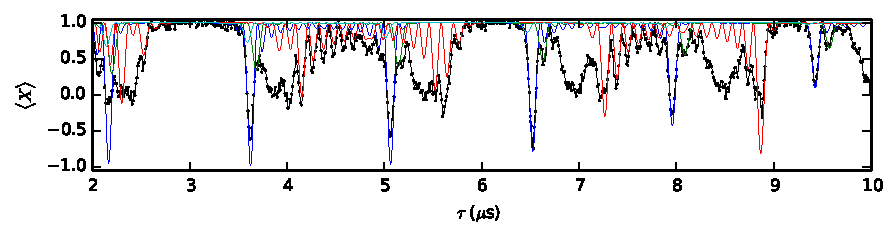
\includegraphics{Img/fingerprint16.pdf}};
            \node[font=\small, text = blue] at (4.05,1.7)  {1};
            \node[font=\small, text = green] at (9.3,2.9) {2};
            \node[font=\small, text = red] at (5.3,2.5) {3};
            \node[font=\small, text = cyan] at (4.0,3.35) {4};
            % \draw[help lines,xstep=1,ystep=1] (0,0) grid (10,3);
            % \foreach \x in {1,2,...,10} { \node [anchor=north] at (\x,0) {\x}; }
            % \foreach \y in {1,2,...,3} { \node [anchor=east] at (0,\y) {\y}; }
        \end{tikzpicture}
        \label{fig:FP16}
    \end{subfigure}

    \begin{subfigure}[t]{\textwidth}\centering

    \caption{}
    \begin{tikzpicture}
        \node[anchor=south west,inner sep=0] at (0,0) {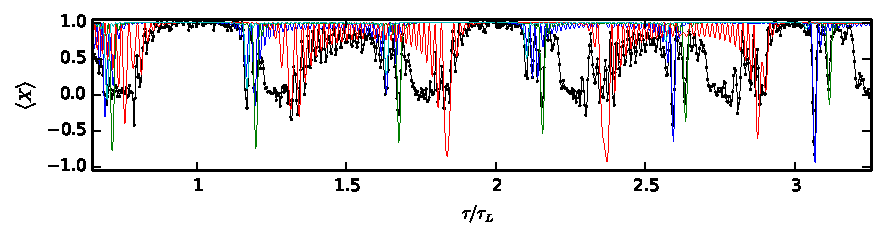
\includegraphics{Img/fingerprint32.pdf}};
        \node[font=\small, text = blue] at (11.2,1.9) {1};
        \node[font=\small, text = blue] at (4.0,2.8)  {1};
        \node[font=\small, text = green] at (6.6,1.8) {2};
        \node[font=\small, text = red] at (7.4,1.8) {3};
        \node[font=\small, text = cyan] at (4.05,2.5) {4};
        % \draw[help lines,xstep=1,ystep=1] (0,0) grid (10,3);
        % \foreach \x in {1,2,...,10} { \node [anchor=north] at (\x,0) {\x}; }
        % \foreach \y in {1,2,...,3} { \node [anchor=east] at (0,\y) {\y}; }
    \end{tikzpicture}
    \label{fig:FP32}
    \end{subfigure}
    \caption{Part of a fingerprint resulting from a dynamical-decoupling-spectroscopy experiment performed at 304G. A reference to the full spectroscopy can be found in \cref{chap:Fingerprint_data_appendix}.  Colored lines represent computed responses of carbon spins. Responses were calculated using \cref{eq:contrast_single_carbon_spin} with hyperfine parameters from \cref{tbl:HF_par}. }
    \label{fig:FP}
\end{figure}
